\documentclass{beamer}
\usepackage[style=verbose,backend=biber]{biblatex}
\addbibresource{SlideDeck.bib}

\renewbibmacro{in:}{}
\beamertemplatenavigationsymbolsempty
\newcommand{\upperRomannumeral}[1]{\uppercase\expandafter{\romannumeral#1}}

\setbeamertemplate{frametitle}{\nointerlineskip  
    \vspace*{3ex} \insertframetitle \hfill {\footnotesize\insertframenumber} \hspace*{0.0001em}}

\begin{document}
  \begin{frame}
    \frametitle{Reservoir modeling of Carbon through Deep Time}
  \end{frame}

  \begin{frame}
    \frametitle{Key reservoirs of carbon today \upperRomannumeral{1}}
    \begin{table}
        \centering
        \begin{tabular}{|l|l|c|c|}
            \hline
            Reservoir & Mass of carbon Gt & Reference \\
            \hline
            Core   & $4 \times 10^9$ & ~\footcite{DR:2013}  \\
            \hline
            Mantle & $2 \times 10^8$ & ~\footcite{KLH-TDL-WM:2018}  \\
            \hline
            Continental crust & $4.2 \times 10^7$ & ~\footcite{KHW:1995} \\
            \hline
            Oceans & $3.8 \times 10^4$ & ~\footcite{HRA:2007} \\
            \hline
            Atmosphere & $8.5 \times 10^2$ & ~\footcite{NOAA:2017} \\
            \hline
            Total & $4.24 \times 10^9$ & \\
            \hline
        \end{tabular}
        \caption{Masses of carbon in the Earth's carbon reservoirs considered in this paper (1 Gt $= 10^{12}$ kg).
        }
        \label{Table:Masses of carbon in Earth's reservoirs}
    \end{table}

  \end{frame}

  \begin{frame}
    \frametitle{Key reservoirs of carbon today \upperRomannumeral{2}}
    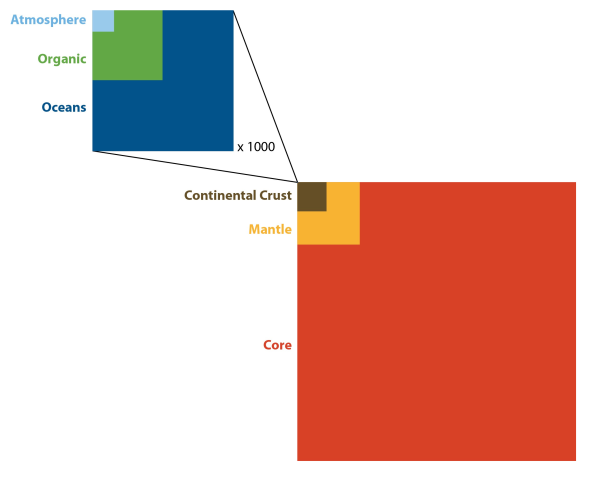
\includegraphics[scale=0.5]{Figures/relative_size_of_reservoirs}
    \footcite{KLH-TDL-WM:2018}
  \end{frame}

  \begin{frame}
    \frametitle{Pathways between reservoirs}
  \end{frame}

  \begin{frame}
    \frametitle{Problems and Complexities}
  \end{frame}

  \begin{frame}
    \frametitle{Model demo}
  \end{frame}
\end{document}
